\FloatBarrier
\subsection{RLS identification with noise on output}

The Simulink model for the system, which uses a combination of sine waves as input and includes white noise on the output, is depicted in \autoref{fig:RLSIWNOSineSimulinModel}. The resulting system output is shown in \autoref{fig:RLSIWNOSineOutput}, and the parameter evaluation during the identification process is presented in \autoref{fig:RLSIWNOSineParams}. The final identified transfer function is given in \autoref{eq:RLSIWNOSineTransferFunction}. The input signal was generated by combining two sine waves, each with an amplitude of 1 and frequencies of $0.1 \frac{rad}{s}$ and $0.07 \frac{rad}{s}$.

\begin{figure}
	\centering
	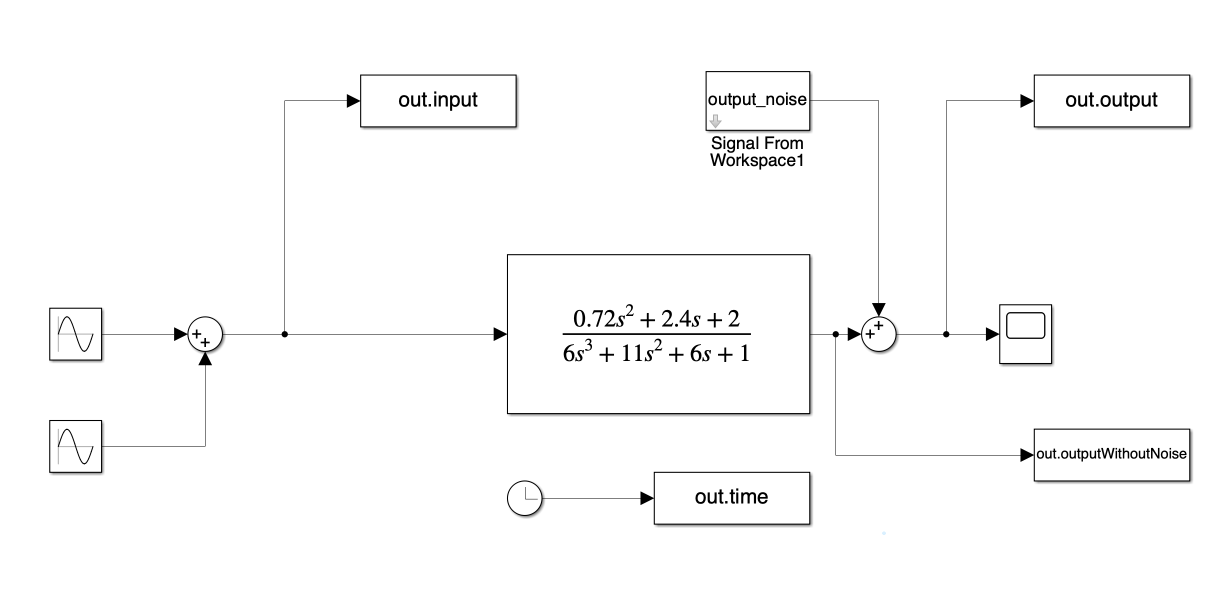
\includegraphics[totalheight=8cm]{images/RLSIWNOSineSimulinkModel.png}
	\caption{RLS Simulink model for system with sine input}
	\label{fig:RLSIWNOSineSimulinModel}
\end{figure}

\begin{figure}
	\centering
	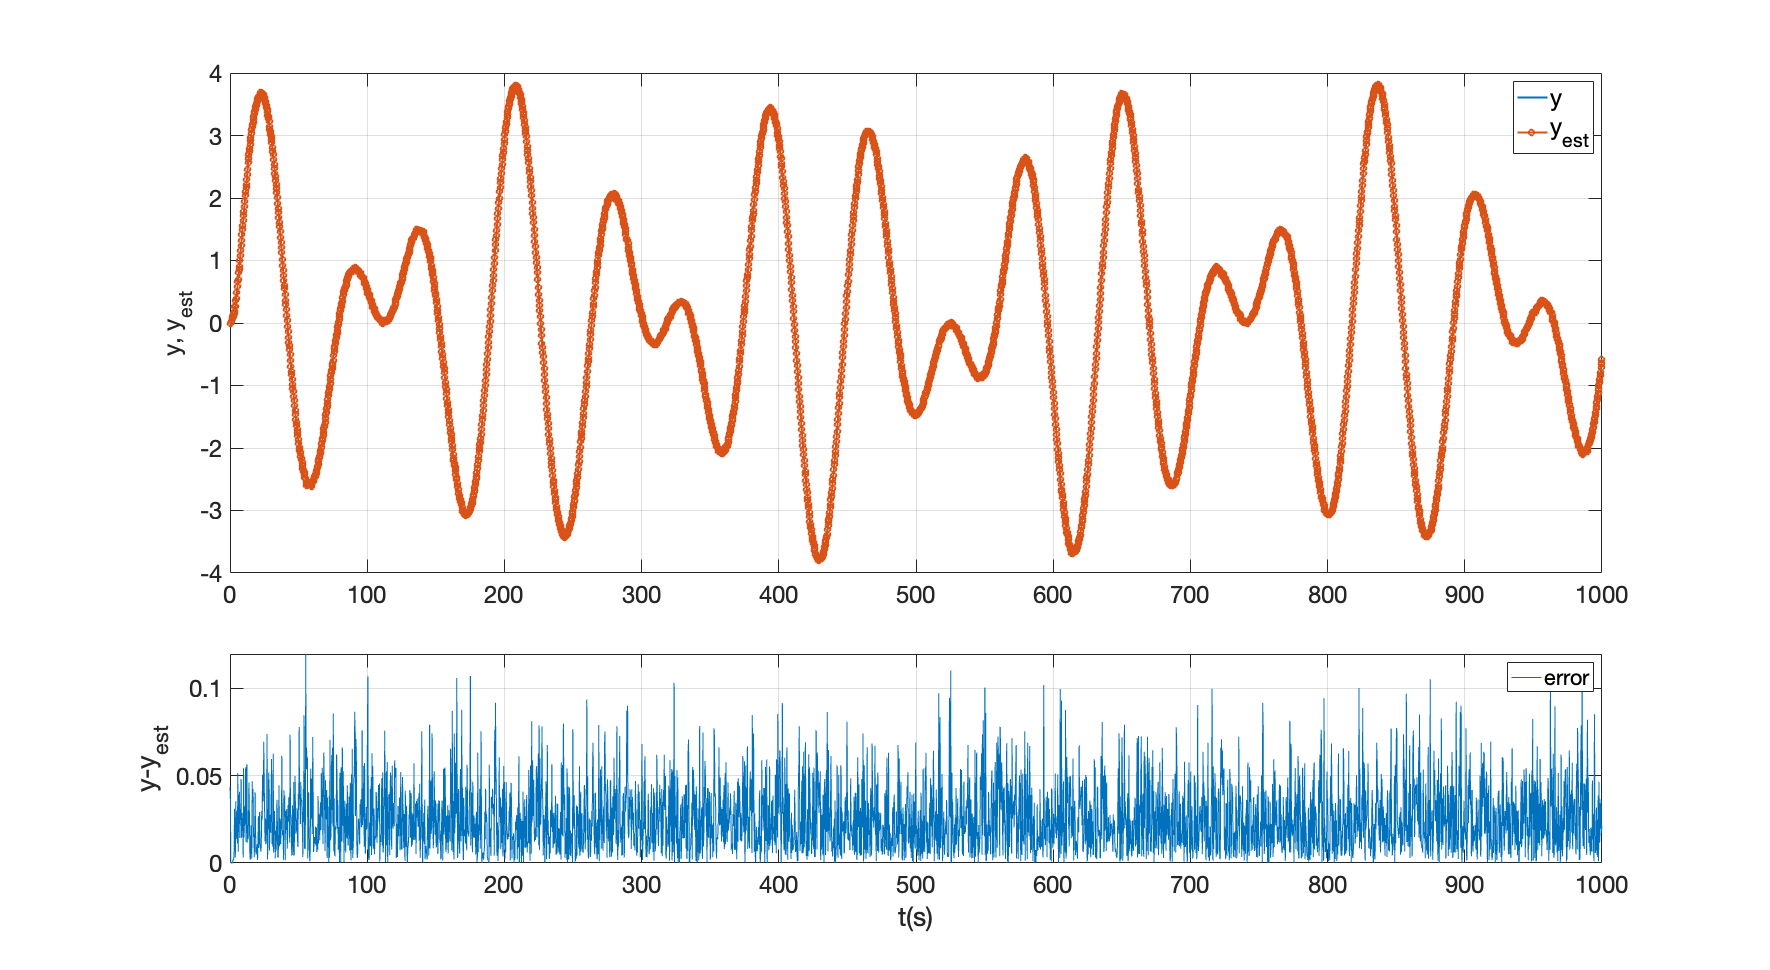
\includegraphics[totalheight=8cm]{images/RLSIWNOSineOutput.png}
	\caption{RLS system output comparison for sine input \& white noise on output}
	\label{fig:RLSIWNOSineOutput}
\end{figure}

\begin{figure}
	\centering
	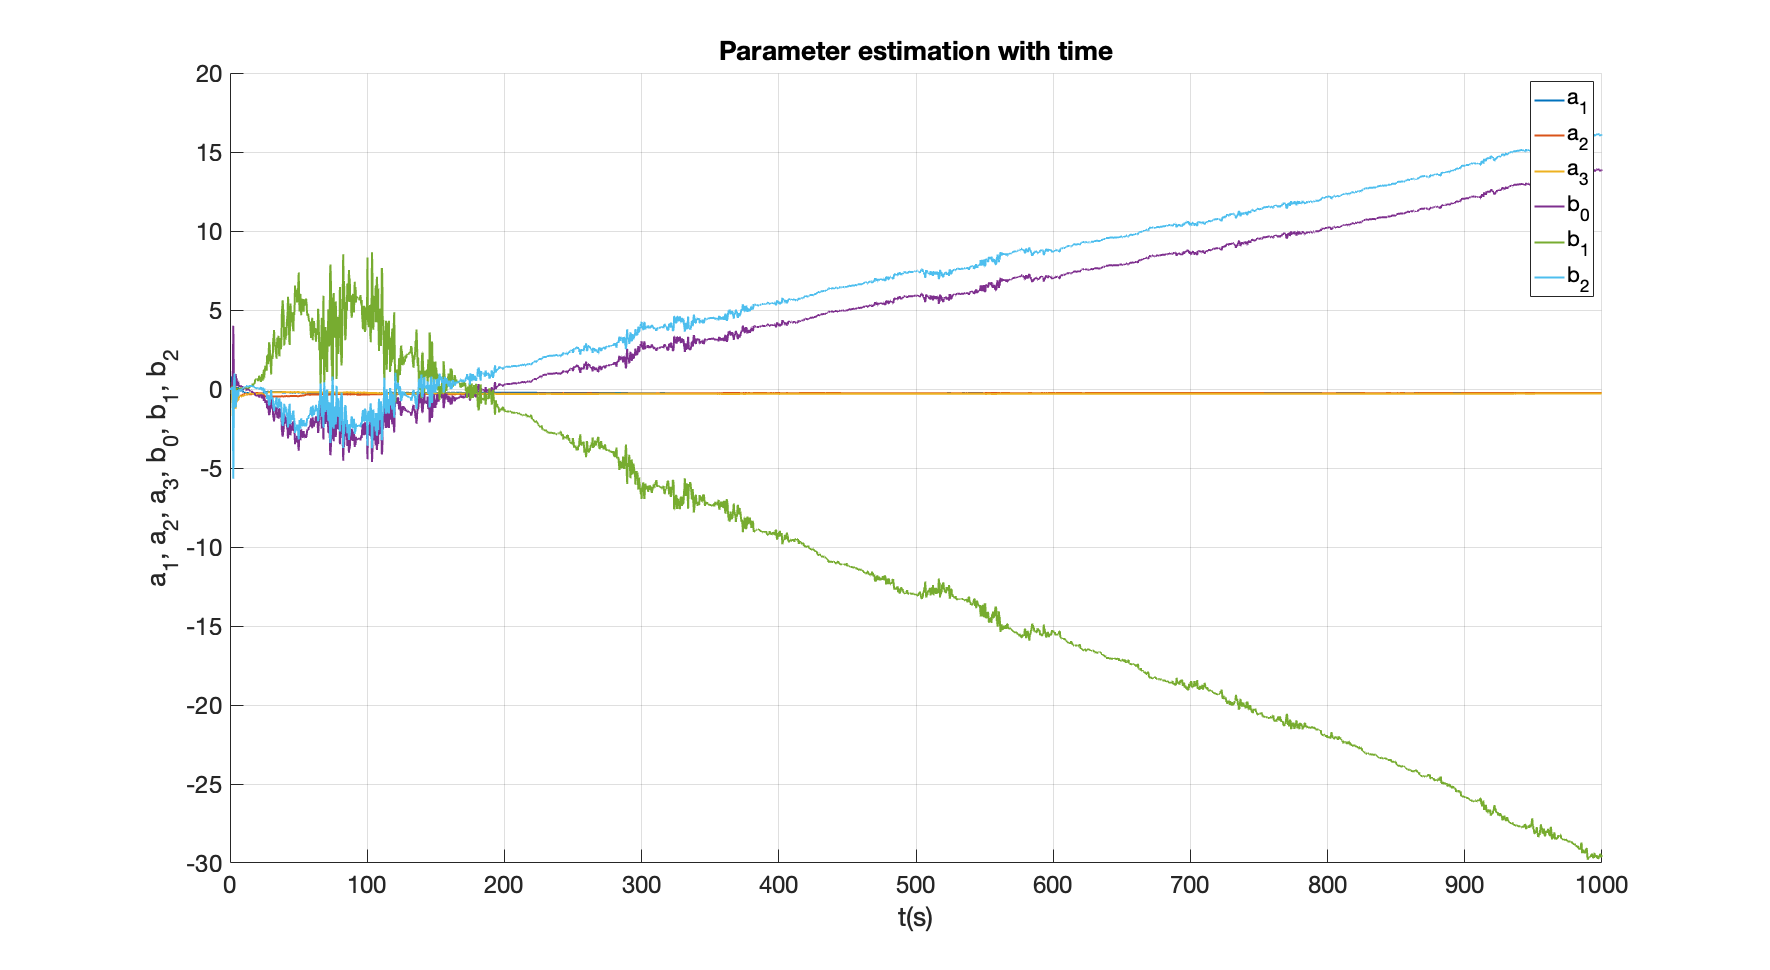
\includegraphics[totalheight=8cm]{images/RLSIWNOSineParams.png}
	\caption{RLS system parameters for sine input \& white noise on output}
	\label{fig:RLSIWNOSineParams}
\end{figure}

\begin{equation}
	G(z) =	\frac{ 13.82 z^2 - 29.5 z + 16.05}{z^3 - 0.2701 z^2 - 0.2535 z - 0.2891}
	\label{eq:RLSIWNOSineTransferFunction}
\end{equation}

The Simulink model designed for the system with a sine wave input is available at \lstinline|assignment1/part2/2_2/RLS2_2_SN.slx|, while the corresponding MATLAB code used for this system is located at \lstinline|assignment1/part2/2_2/RLS2_2_sine.m|.


For the system with white noise input, we used the same Simulink model as in \autoref{fig:LSIWNONoiseSimulinkModel}. The system's output and parameter evaluation are shown in \autoref{fig:RLSIWNOWhiteNoiseOutput} and \autoref{fig:RLSIWNOWhiteNoiseParams}, respectively. The resulting transfer function is given by \autoref{eq:RLSIWNOWhiteNoiseTransferFunction}.

\begin{figure}
	\centering
	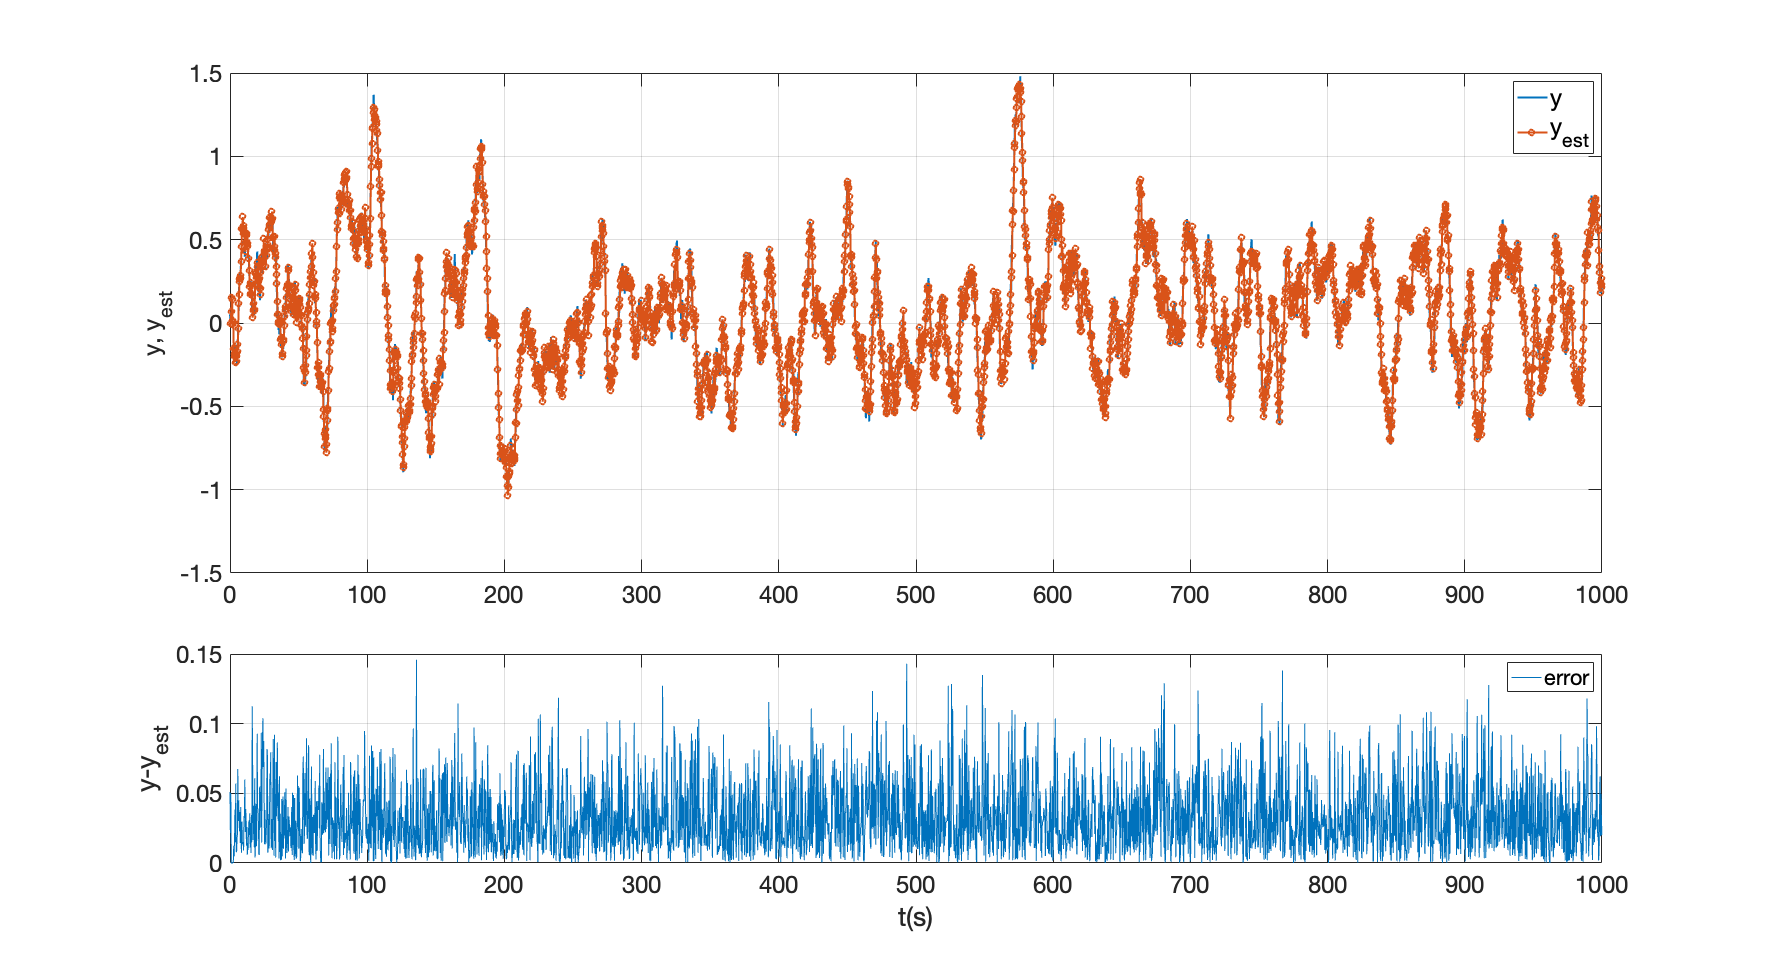
\includegraphics[totalheight=8cm]{images/RLSIWNOWhiteNoiseOutput.png}
	\caption{RLS system output comparison for white noise on input \& output}
	\label{fig:RLSIWNOWhiteNoiseOutput}
\end{figure}

\begin{figure}
	\centering
	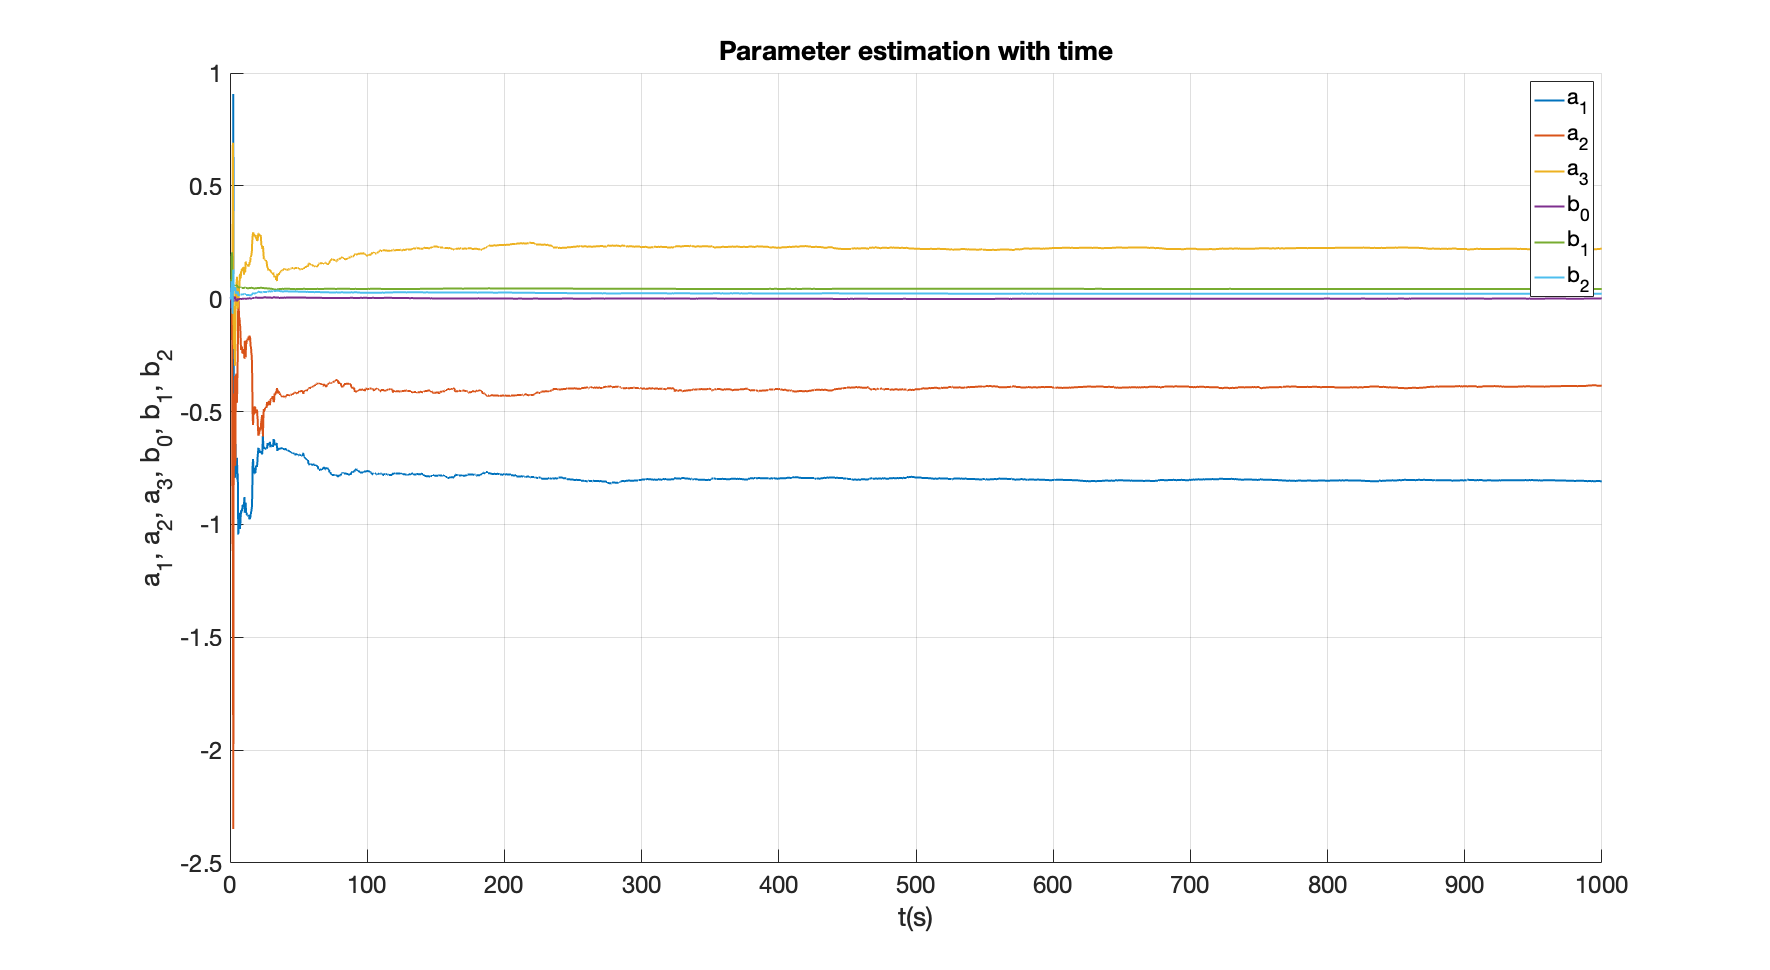
\includegraphics[totalheight=8cm]{images/RLSIWNOWhiteNoiseParams.png}
	\caption{RLS system parameters for white noise on input \& output}
	\label{fig:RLSIWNOWhiteNoiseParams}
\end{figure}

\begin{equation}
	G(z) =	\frac{ 0.0004192 z^2 + 0.04334 z + 0.02165}{z^3 - 0.8084 z^2 - 0.3853 z + 0.2211}
	\label{eq:RLSIWNOWhiteNoiseTransferFunction}
\end{equation}

The Simulink model for the system with white noise input can be accessed at \hspace{-1ex}\lstinline| assignment1/part2/2_2/RLS2_2_NS.slx|.
Matlab code for the system is at \hspace{-1ex}\lstinline| assignment1/part2/2_2/RLS2_2_noise.m|.